\section{Free Body Diagrams}

Free body diagrams are a method of communicating the application and direction of forces through an object. The objective is to simplify the geometry of an object to a point where one can easily see how the forces within the object interact with one another. It is also common practice to take planes in which the forces are acting to reduce the complexity of the interaction of forces further.

\cref{fig-fbd} shows an example of a loaded beam whose forces have been split in both the horizontal and vertical directions, and are reacted by two bearings. The $+$ arrow indicates our sign convention on the drawing and relative positions of the forces are also indicated.

\begin{figure*}[ht!]
  \center
  \begin{tabular}{c c}
    \subfloat[Vertical]{
    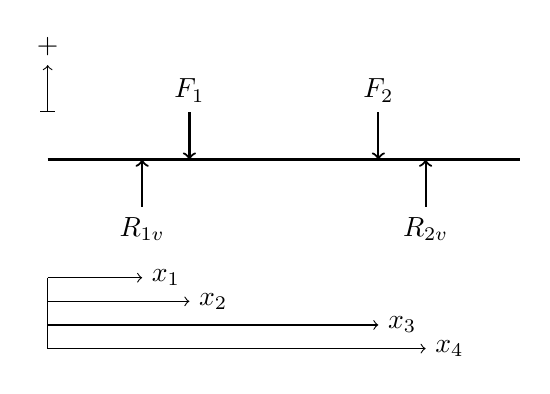
\begin{tikzpicture}[scale=6.0]
      \draw[very thick] (0,0) -- (1,0);
      
      \draw[<-, thick] (0.2,0) -- (0.2,-0.1) node[below]{$R_{1v}$};
      \draw[<-, thick] (0.8,0) -- (0.8,-0.1) node[below]{$R_{2v}$};
      
      \draw[<-, thick] (0.3,0) -- (0.3,0.1) node[above]{$F_{1}$};
      \draw[<-, thick] (0.7,0) -- (0.7,0.1) node[above]{$F_{2}$};
      
      \draw[->] (0,-0.25) -- (0.2,-0.25) node[right]{$x_1$};
      \draw[->] (0,-0.3) -- (0.3,-0.3) node[right]{$x_2$};
      \draw[->] (0,-0.35) -- (0.7,-0.35) node[right]{$x_3$};
      \draw[->] (0,-0.4) -- (0.8,-0.4) node[right]{$x_4$};
      \draw[] (0,-0.25) -- (0,-0.4);
      
      \draw[|->] (0,0.1) -- (0,0.2) node[above]{$+$};
    \end{tikzpicture}
  } &
  \subfloat[Horizontal]{
    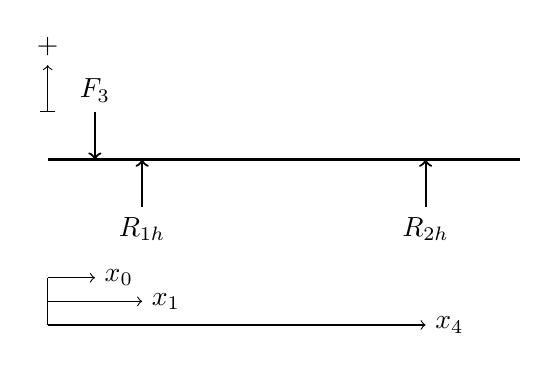
\begin{tikzpicture}[scale=6.0]
      \draw[very thick] (0,0) -- (1,0);
      
      \draw[<-, thick] (0.2,0) -- (0.2,-0.1) node[below]{$R_{1h}$};
      \draw[<-, thick] (0.8,0) -- (0.8,-0.1) node[below]{$R_{2h}$};
      
      \draw[<-, thick] (0.1,0) -- (0.1,0.1) node[above]{$F_{3}$};
      
      \draw[->] (0,-0.25) -- (0.1,-0.25) node[right]{$x_0$};
      \draw[->] (0,-0.3) -- (0.2,-0.3) node[right]{$x_1$};
      \draw[->] (0,-0.35) -- (0.8,-0.35) node[right]{$x_4$};
      \draw[] (0,-0.25) -- (0,-0.35);
      
      \draw[|->] (0,0.1) -- (0,0.2) node[above]{$+$};
    \end{tikzpicture}
  } \\
  \end{tabular}
  \vspace{1em}
  \caption{Free-body diagrams for a loaded beam}\label{fig-fbd}
\end{figure*}

Using these diagrams and information on the forces and location of the forces, one can ascertain the reactions on the bearings.

\begin{multicols}{4}
\begin{description}
    \item[$F_1$] = \SI{15}{\kilo\newton}
    \item[$F_2$] = \SI{25}{\kilo\newton}
    \item[$F_3$] = \SI{10}{\kilo\newton}
    \item[$R_{1v}$] = ?
    \item[$R_{1h}$] = ?
    \item[$R_{2v}$] = ?
    \item[$R_{2h}$] = ?
    \item[$x_0$] = \SI{0}{\metre}
    \item[$x_1$] = \SI{0.2}{\metre}
    \item[$x_2$] = \SI{0.3}{\metre}
    \item[$x_3$] = \SI{0.55}{\metre}
    \item[$x_4$] = \SI{0.6}{\metre}
\end{description}
\end{multicols}

To\marginnote{Resolving the Vertical Forces}  resolve the force vertically, we take moments about one of the bearings with the assumption that it is a static and stable system. Thus, no moment should exist about the bearing otherwise the shaft would be spinning!

Here, we have taken moments about $R_{1v}$ and from this, we can calculate the reaction force $R_{2v}$. 
\begin{align}
  \circlearrowright R_{1v} &= 0 = \SI{0.1}{\metre}(\SI{15}{\kilo\newton}) + \SI{0.35}{\metre}(\SI{25}{\kilo\newton}) - 0.4(R_{2v}) \\
  R_{2v} &= \frac{\SI{1025}{\kilo\newton\metre}}{\SI{0.4}{\metre}} = \SI{25.625}{\kilo\newton}
\end{align}

With $R_{2v}$ calculated, we can look at the balancing the forces in the vertical plane to ascertain $R_{1v}$.
\begin{align}
  R_{1v}+R_{v2}&=F_1+F_2\\
  R_{1v}+R_{v2}&=\SI{15}{\kilo\newton}+\SI{25}{\kilo\newton}\\
  R_{1v} &= \SI{40}{\kilo\newton}-\SI{25.625}{\kilo\newton} = \SI{14.375}{\kilo\newton}
\end{align}

The\marginnote{Resolving the Horizontal Forces} same process used in the horizontal direction. Taking moments about $R_{1h}$, we can find $R_{2h}$.
\begin{align}
  \circlearrowright R_{1h} &= 0 = \SI{0.2}{\metre}(\SI{10}{\kilo\newton}) + 0.4\si{\metre}(R_2) \\
  \therefore R_{2h} &=  \frac{0.2\si{\metre}}{-0.4\si{\metre}} = -5\si{\kilo\newton}
\end{align}

Again, equating the forces in the horizontal plane gives us $R_{1h}$.
\begin{align}
  R_{1h}+R_{2h}&=\SI{10}{\kilo\newton} \\
  R_{1h} &= \SI{10}{\kilo\newton} + \SI{5}{\kilo\newton} = \SI{15}{\kilo\newton}
\end{align}

